% !TeX root = ../../thesis.tex
\chapter{This is introduction}\label{ch:introduction}

\instructionsintroduction

% Illustration on how to refer to your papers when using biblatex
% (see second line in thesis.tex to activate biblatex)
%\definecolor{shadecolor}{gray}{0.85}
%\begin{shaded}
%This chapter was previously published as:\\
%\fullcite{VandenBroeck2011IJCAI}
%\newpage
%\end{shaded}

% Some dummy code to make sure bibtex does not complain.
Illustration of how to include citations \cite{Meert2011PhD} and \cite{VandenBroeck2011IJCAI}. Lorem ipsum dolor sit amet, consetetur sadipscing elitr, sed diam nonumy eirmod tempor invidunt ut labore et dolore magna aliquyam erat, sed diam voluptua. At vero eos et accusam et justo duo dolores et ea rebum. Stet clita kasd gubergren, no sea takimata sanctus est Lorem ipsum dolor sit amet.

And yet another citation \cite{FrRo2010Diffusion}.

% Some dummy code to get at least 1 entry in the nomenclature.
\nomenclature{$\Theta$}{A nice symbol}
Introducing some symbol: $\Theta$.

% Some dummy code to get at least 1 entry in the list of
% abbreviations.
\newglossaryentry{md}{name={MD},description={molecular dynamics}}
Introducing an acronym: \gls{md}.

% Some dummy code show how to include images.
\begin{figure}
  \centering
  \medskip
  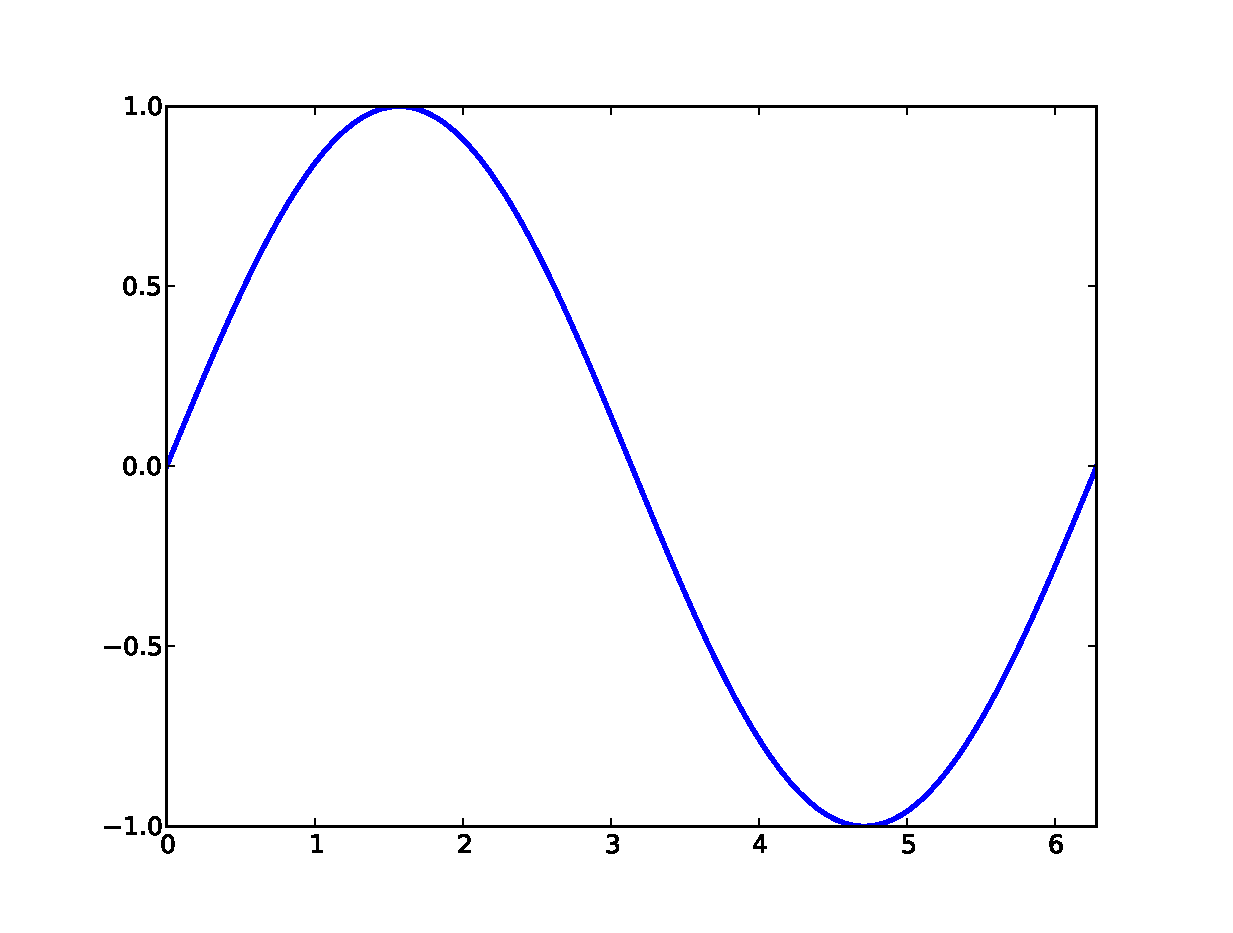
\includegraphics[width=.9\textwidth]{sine}
  \caption[Short caption for Table of Figures]{Illustration of how to
  include a figure (long text, should not go to Table of Figures).}
  \label{fig:sine}
\end{figure}

There is a small change here.




%%%%%%%%%%%%%%%%%%%%%%%%%%%%%%%%%%%%%%%%%%%%%%%%%%
% Keep the following \cleardoublepage at the end of this file, 
% otherwise \includeonly includes empty pages.
\cleardoublepage

% vim: tw=70 nocindent expandtab foldmethod=marker foldmarker={{{}{,}{}}}
